% Problem description section
\begin{frame}{Problem description}
    \begin{block}{T-Shirt distribution problem}
        You are a T-Shirt distributor and want to optimise your packaging
        process when sending boxes of T-Shirts to stores.
    \end{block}
    \only<1>{
        \begin{center}
            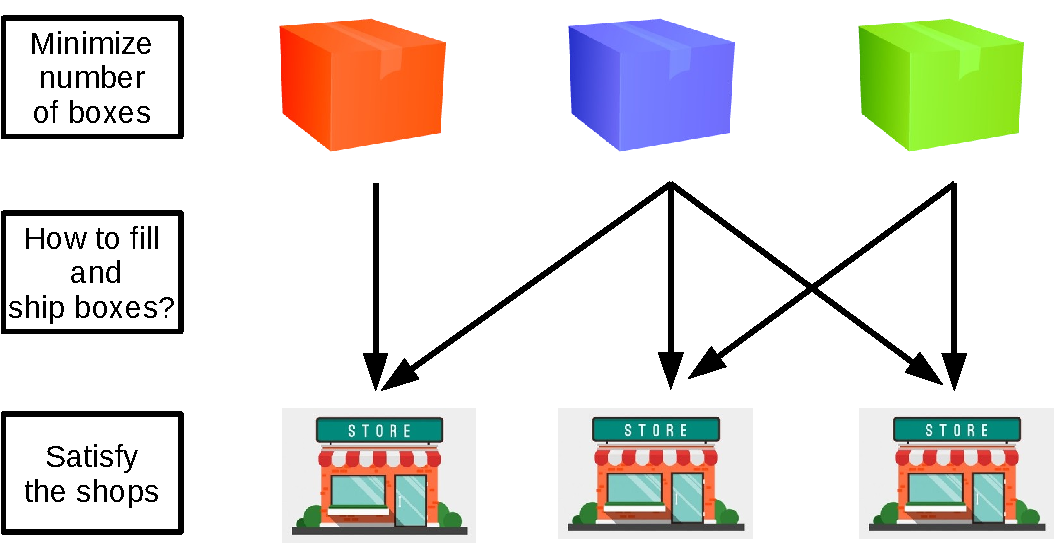
\includegraphics[width=0.75\textwidth]{./figures/problem-overview-crop.pdf}
        \end{center}
    }
    \only<2>{
    \begin{itemize}
        \item It is expensive to train your staff on packing T-Shirts into many
        different types of boxes.
        \item Each store requires a
        certain number of T-Shirts of given sizes.
        \item Stores will only accept receiving more T-Shirts than ordered in the case of
        medium and large Shirts in colors black, blue or red.
        \item Over-stocking is bad, but under-stocking is a lot (say $10$ times) worse.
        \item You are supplied with boxes that fit 4, 6, 8
        or 10 T-Shirts and can not ship partially filled boxes.
        \item You offer a total of $24$ different T-Shirts.\\
            \hfill(Six different sizes offered in four different colors)
    \end{itemize}}
\end{frame}

\begin{frame}{Optimisation problem}
    Variables in the optimisation problem
    \begin{align*}
        \text{Orders: }& \text{o}_i \in \N_{\geq 0}^{24}\\
        \text{Boxes: }& \text{b}_j \in \N_{\geq 0}^{24}, \text{ with }
        \text{b}_j^T 1 \in \{4, 6, 8, 10\}, \text{ for all } j \in 1,...,M\\
        \text{Delivery plan: }& \alpha_{(i,j)}\in \N_{\geq 0}~ \forall i, j\\
        \text{Deliveries: }& \text{s}_i =
        \sum_{j = 1,\dots,M}\alpha_{(i,j)}\text{b}_j~\text{ for all } j \in 1,\dots,58\\
    \end{align*}
    Where $\alpha_{i,j}$ is the number of boxes of type $j$ that store $i$ will
    receive and $M$ is the total number of different box-types used.
\end{frame}

\begin{frame}{Formulation as an integer optimisation problem}
    \begin{align*}
        \text{minimize: } & \underbrace{\beta M}_{\text{Penalise number of
        boxes}} + \sum_{i = 1}^{58}
        \underbrace{\mathbbm{1}_{\text{s}_i > \text{o}_i} (\text{s}_i -
        \text{o}_i)}_{\text{Penalise overstocking}} +
        \underbrace{
            10 \cdot \mathbbm{1}_{\text{s}_i < \text{o}_i}(\text{o}_i -
            \text{s}_i)}_{\text{Penalise understocking more}}\\
        \text{subject to:}&\\
        &\text{M} \in \N_{\geq 1}\\
        &\text{b}_j \in \N_{\geq 0}^{24}~\forall~j = 1,\dots,M\\
        &\alpha_{(i,j)} \in \N_{\geq 0}^{24}~\forall~i=1,\dots,58,~j=1,\dots,M\\
        &\text{s}_i = \sum_{j = 1,\dots,M}\alpha_{(i,j)}\text{b}_j \leq
        \text{o}_i^{\text{limit}}~\forall~i = 1,\dots,58\\
    \end{align*}
    \begin{itemize}
        \item Note: Optimal solution depends on penalty parameter $\beta > 0$.\\
        \item In general integer optimisation problems are NP-Hard.\\
    \end{itemize}

\end{frame}
